% !TEX TS-program = pdflatex
% !TEX encoding = UTF-8 Unicode


%%%%%%%%%%%%%%%%%%%%%%%%%%%%%%%%%%%%%%%%%%%%%%%%%%%%%%%%%%%%%%%%%%%%%%%%%%%%%%%%
%%%%%%%%                        DOCUMENT PREAMBLE                       %%%%%%%%
%%%%%%%%%%%%%%%%%%%%%%%%%%%%%%%%%%%%%%%%%%%%%%%%%%%%%%%%%%%%%%%%%%%%%%%%%%%%%%%%

\documentclass[12pt]{article}

\usepackage[utf8]{inputenc}

%%% PAGE DIMENSIONS
\usepackage{geometry}
\geometry{a4paper}
\geometry{margin=1in}

%%% PACKAGES
\usepackage{booktabs} 		% for much better looking tables
\usepackage{array} 			% for better arrays (eg matrices) in maths
\usepackage{paralist} 		% very flexible & customisable lists (eg. enumerate/itemize, etc.)
\usepackage{verbatim} 		% adds environment for commenting out blocks of text & for better verbatim
\usepackage{caption}
\usepackage{subcaption} 		% make it possible to include more than one captioned figure/table in a single float
\usepackage{amsmath}		% gives math environments like align, split, etc
\usepackage[parfill]{parskip} % Activate to begin paragraphs with an empty line rather than an indent
\usepackage{xcolor}			% adds support for different colors
\usepackage{float}			% adds support for floats
\usepackage{upgreek}		% greek letters
\usepackage{amssymb}
\usepackage{url}
\usepackage[binary-units]{siunitx}
\usepackage{pdfpages}

%%% Images
\usepackage{graphicx}		% allows us to include images
\graphicspath{ {./images/} }


%%% HEADERS & FOOTERS
\usepackage{fancyhdr} 		% This should be set AFTER setting up the page geometry
\pagestyle{fancy}
\renewcommand{\headrulewidth}{0pt} % customise the layout...
\lhead{}\chead{}\rhead{}
\lfoot{}\cfoot{\thepage}\rfoot{}


%%% ToC (table of contents) APPEARANCE
% \usepackage[nottoc,notlof,notlot]{tocbibind} % Put the bibliography in the ToC
% \usepackage[titles,subfigure]{tocloft} % Alter the style of the Table of Contents
% \renewcommand{\cftsecfont}{\rmfamily\mdseries\upshape}
% \renewcommand{\cftsecpagefont}{\rmfamily\mdseries\upshape} % No bold!


%%% Referencing and Bibliography
\usepackage[backend=bibtex, style=ieee]{biblatex}
\addbibresource{references.bib}


%%% Title Stuff
\title{ENCE461 Assignment 2}
\author{
	J.P. Sheehan \\
	M.F. Hamblyn \\
	\small{Group 36}
}
\date{\today}



%%%%%%%%%%%%%%%%%%%%%%%%%%%%%%%%%%%%%%%%%%%%%%%%%%%%%%%%%%%%%%%%%%%%%%%%%%%%%%%%
%%%%%%%%                          DOCUMENT BODY                         %%%%%%%%
%%%%%%%%%%%%%%%%%%%%%%%%%%%%%%%%%%%%%%%%%%%%%%%%%%%%%%%%%%%%%%%%%%%%%%%%%%%%%%%%

\begin{document}
\maketitle
\thispagestyle{empty}

\vfill
\begin{figure}[H]
	\centering
	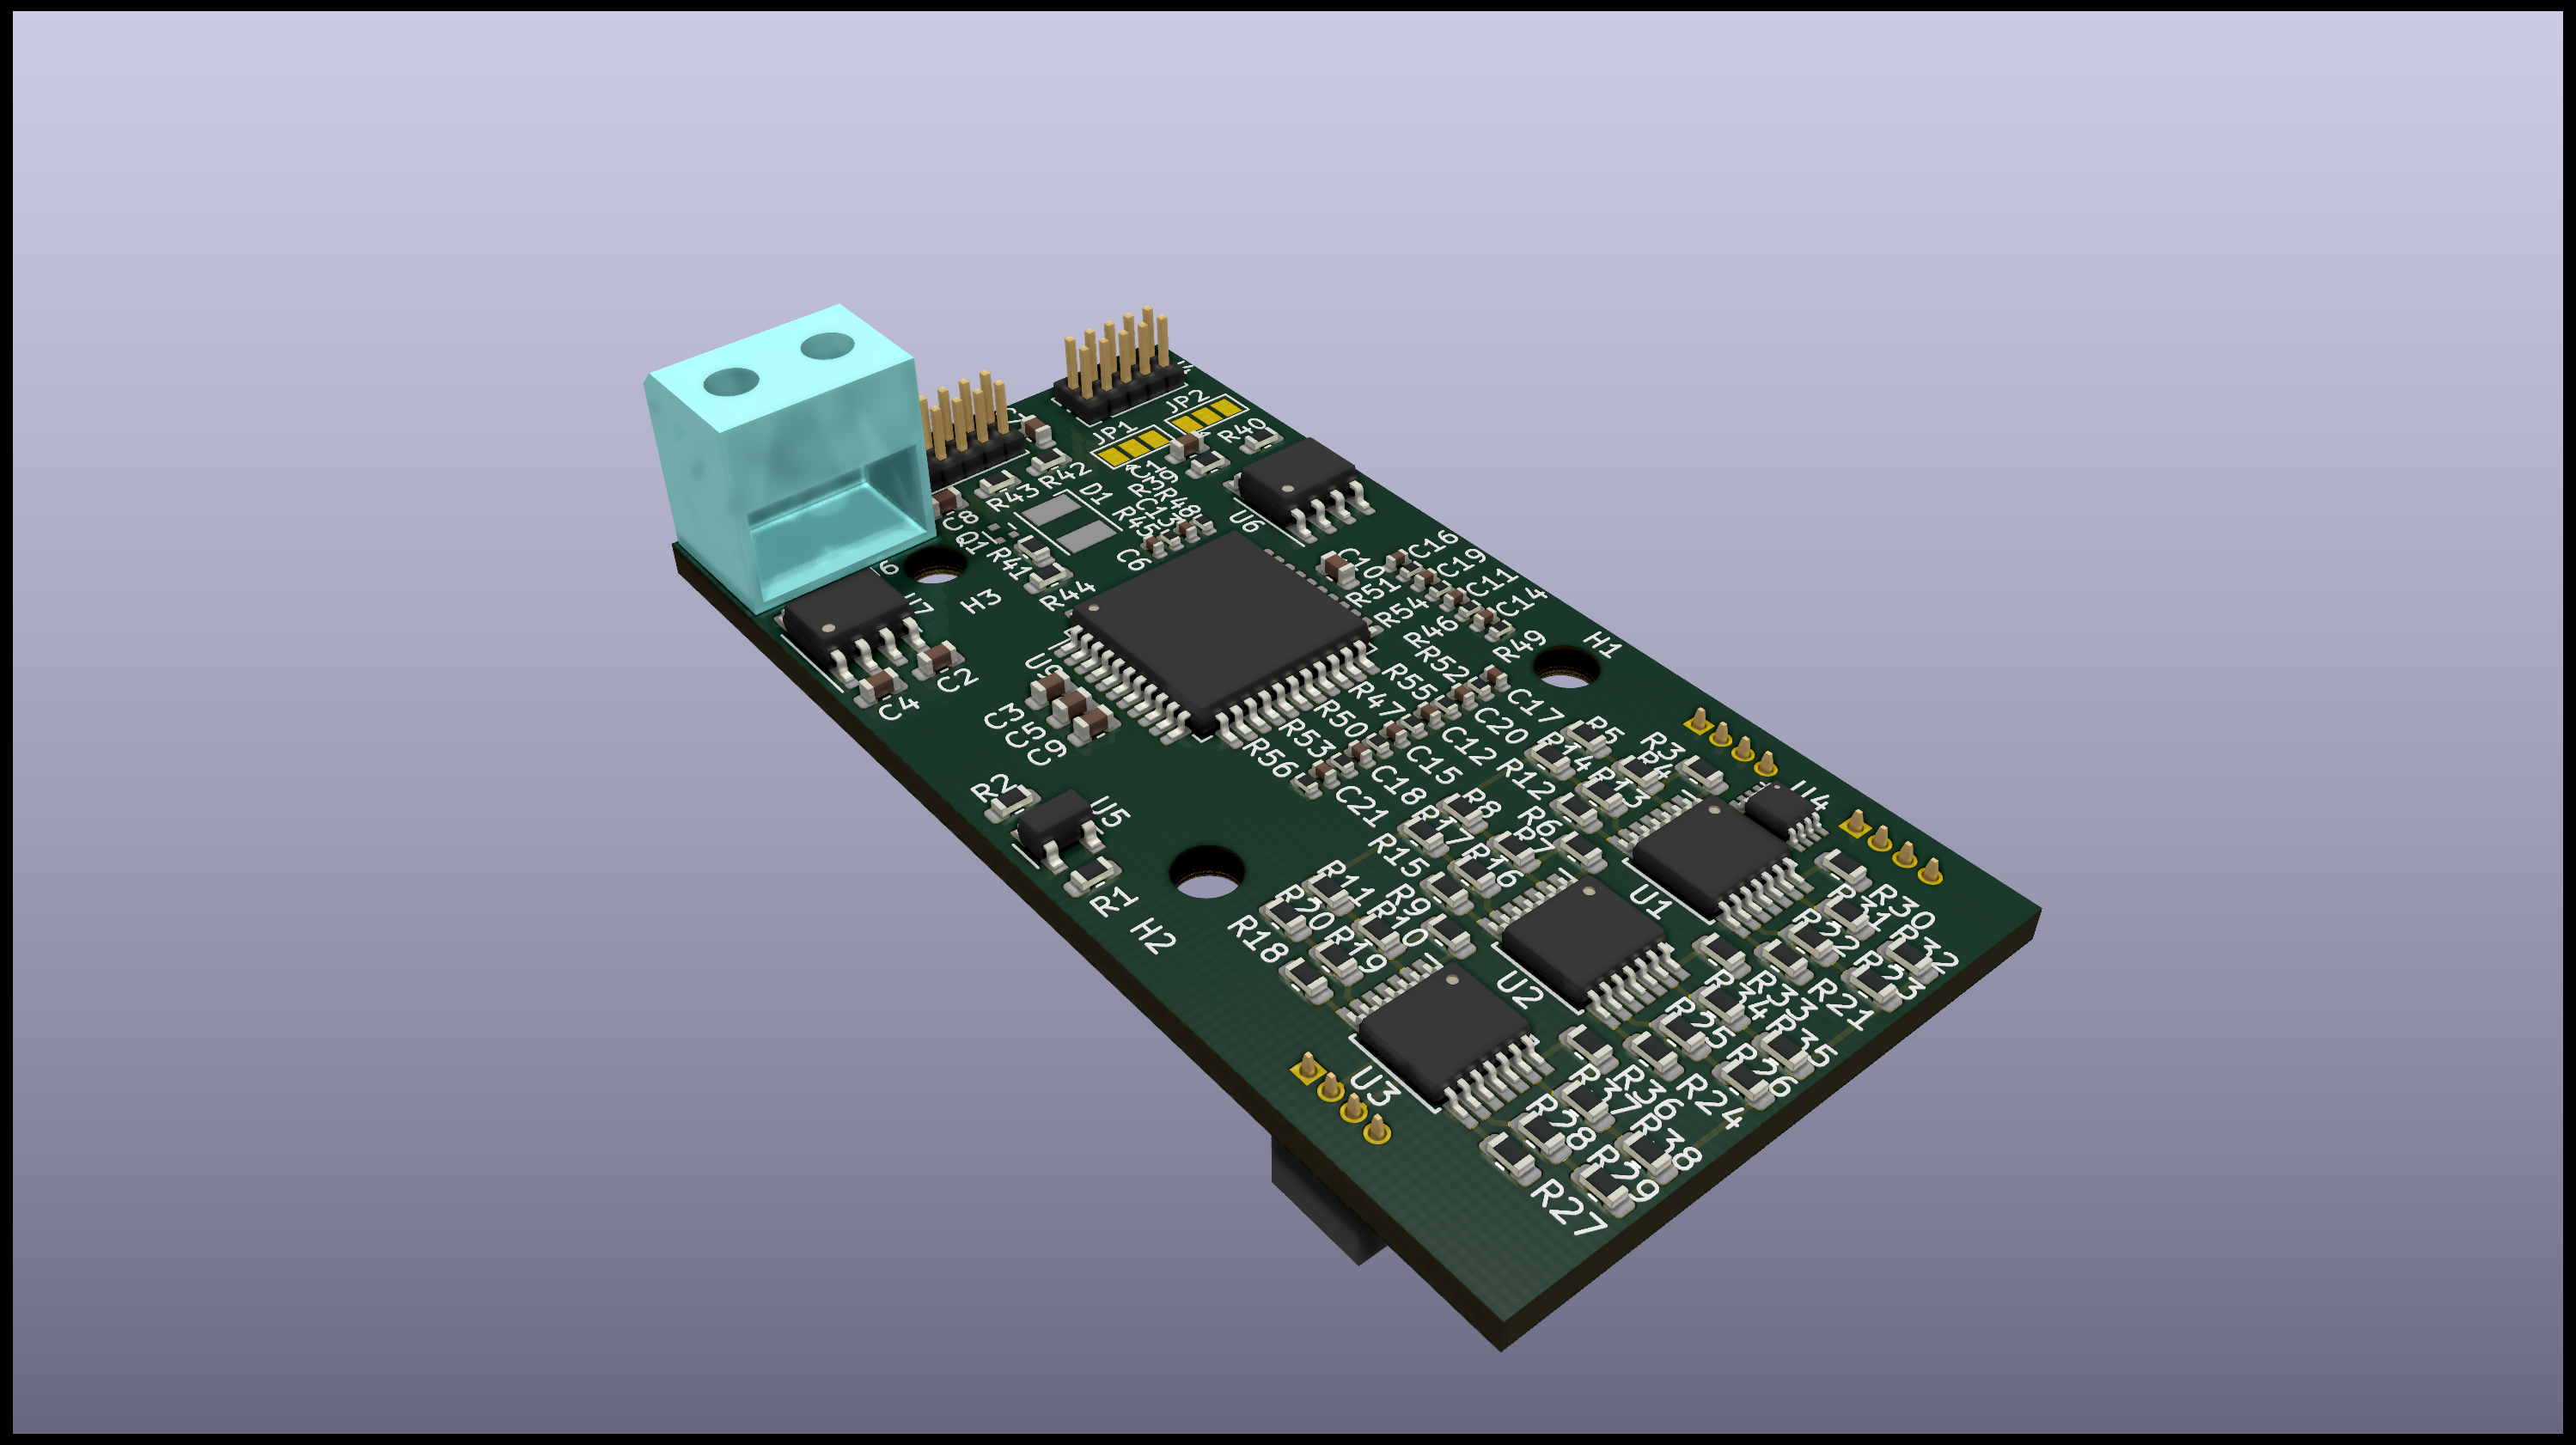
\includegraphics[width=\textwidth]{render}
	\label{fig:render}
\end{figure}
\vfill

\newpage

\section{Introduction}

Based on the provided requirements specifications and subsequnet clarifications the design achieves

\begin{enumerate}
	\item Reliable high speed, multi node, commmunications
	\item Minimal standby mode power consumption
	\item Ease of installation and maintainence 
\end{enumerate}

This following sections outline the key design decisions made with detailed analysis provided in the APPENDIX. 


\section{Design}

\subsection{Power Supply}
Current consumption analysis determined 40 - 90 mA and 70.5 - 110 mA (typical - maximum) are required for the ADC and digital sections respectively. (This rqange is depentant on whether indvidual control of ADC blocks is required, and maximum versues typical consumption values are used.) 
The MIC5202-5.0YMM was selected to provide an independant 5V 100mA output, with disable function, to each section; thus providing the smallest physical footprint and zero ADC current consumption in low power mode. Furrthermore the MIC5202-5.0YMM meets the thermal requirement whereby it's junction temperature must not exceed the reliable operating maximium of 125 degrees when dissapating full current at 105 degres C ambient. Refer to APPENDIX for thermal calculations.
 
\subsection{OpAmp Supply}
The LMV324AIPWR opamp uses 70uA quiescent current. Since the each op amp channel output connects via low pass filter to an MCU ADC input, there is minimal load, thus operating current is small. A conservative value of 2mA per ADC channel has been estimated.
A voltage divider off the 5V ADC rail, with voltage follower op amp, provides the 2.5V half rail reference supply. Divider current is 0.5mA, designed to balence the conflicting requirements of low quiescient current with low value resistors to reduce thermal noise (associated with high ambient temperatures) in the ADC section.
A 3 port hex inverter provides the ability to enable/disable ADC channels in blocks of four and consumes 50mA.

\subsection{MCU Supply}
At 48MHz operation expected current consumption of the ATSAMC21N17A-ANTCT-ND is a conservative 20-30mA, and 25mA has been used foir calculations. The CAN bus transceiver consumes 47 mA typical, 70mA maxlmum.

\subsection{Power modes}
To meet the specification regarding control of ADC channels a 3 port hex inverter is used adding 50mA to the ADC section. If this level of ADC channel selection were not required this could be removed, realising a 50mA standby current saving. With the hex inverter included the following power modes are available:
Mode							Active devices	 					Estimated current consumption.
Sleep. (requires wake)				MCU sleep, CAN standby, ADC off 		<10 mA. 
Low power. 						MCU active, CAN standby, ADC off		<30 mA
Standby. (ready to sample)		MCU active, CAN active, ADC on		<98.5 - <148.5
Sampling.						MCU active, CAN standby, ADC on		51.5 - 100.5 	
Data transfer.					MCU active, CAN active, ADC off		<73

\subsection{Signal Conditioning}

The process of converting the voltage seen at the current transducer to a digital reading involves three stages (figure \ref{fig:conditioning}).
The gain stage amplifies the voltage of the signal up to a reasonable level.
The filtering stage removes any high frequency noise.
Finally, the sampling stage performs the analog to digital (ADC) conversion.
\begin{figure}[H]
	\centering
	
\includegraphics[width=0.8\textwidth]{cat}
	\caption{The signal conditioning process.}
	\label{fig:conditioning}
\end{figure}

\subsubsection{Gain Stage}

The current transducers output a $\pm \SI{25}{\milli\volt}$ signal centered around $\SI{2.5}{\volt}$.
This signal must be amplified to $\pm \SI{2.5}{\volt}$ using an operational amplifier with a gain of 100.
To amplify the signal, a non-inverting op-amp circuit (figure \ref{fig:non-inverting-op-amp}) was used.
12 of these circuits are required for each daughterboard.
The LMV324 was selected as it has four op-amp circuits in one package.
Resistor values of $R_1 = \SI{100}{\kilo\ohm}, R_2 = \SI{1}{\kilo\ohm}, R_3 = \SI{10}{\ohm}$ were chosen to give a gain of $100$ and an input impedance of $\SI{1}{\kilo\ohm}$ for each amplifier circuit.

The half-rail voltage of $\SI{2.5}{\volt}$ is provided by a virtual ground op-amp circuit (figure \ref{fig:half-supply}).
An LMV321 was used for this circuit.
High value resistors are required in the divider (typically $\SI{100}{\kilo\ohm}$ to prevent excessive static current drain.
However, these produce greater thermal noise (especially at high ambient temperatures) which is undesirable for ADC applications.
Therefore, two $\SI{2.5}{\kilo\ohm}$ resistors balance the noise and have a static current drain of $\SI{1}{\milli\ampere}$.

\begin{figure}[ht]
\centering

\begin{subfigure}[c]{0.45\textwidth}
	\centering
	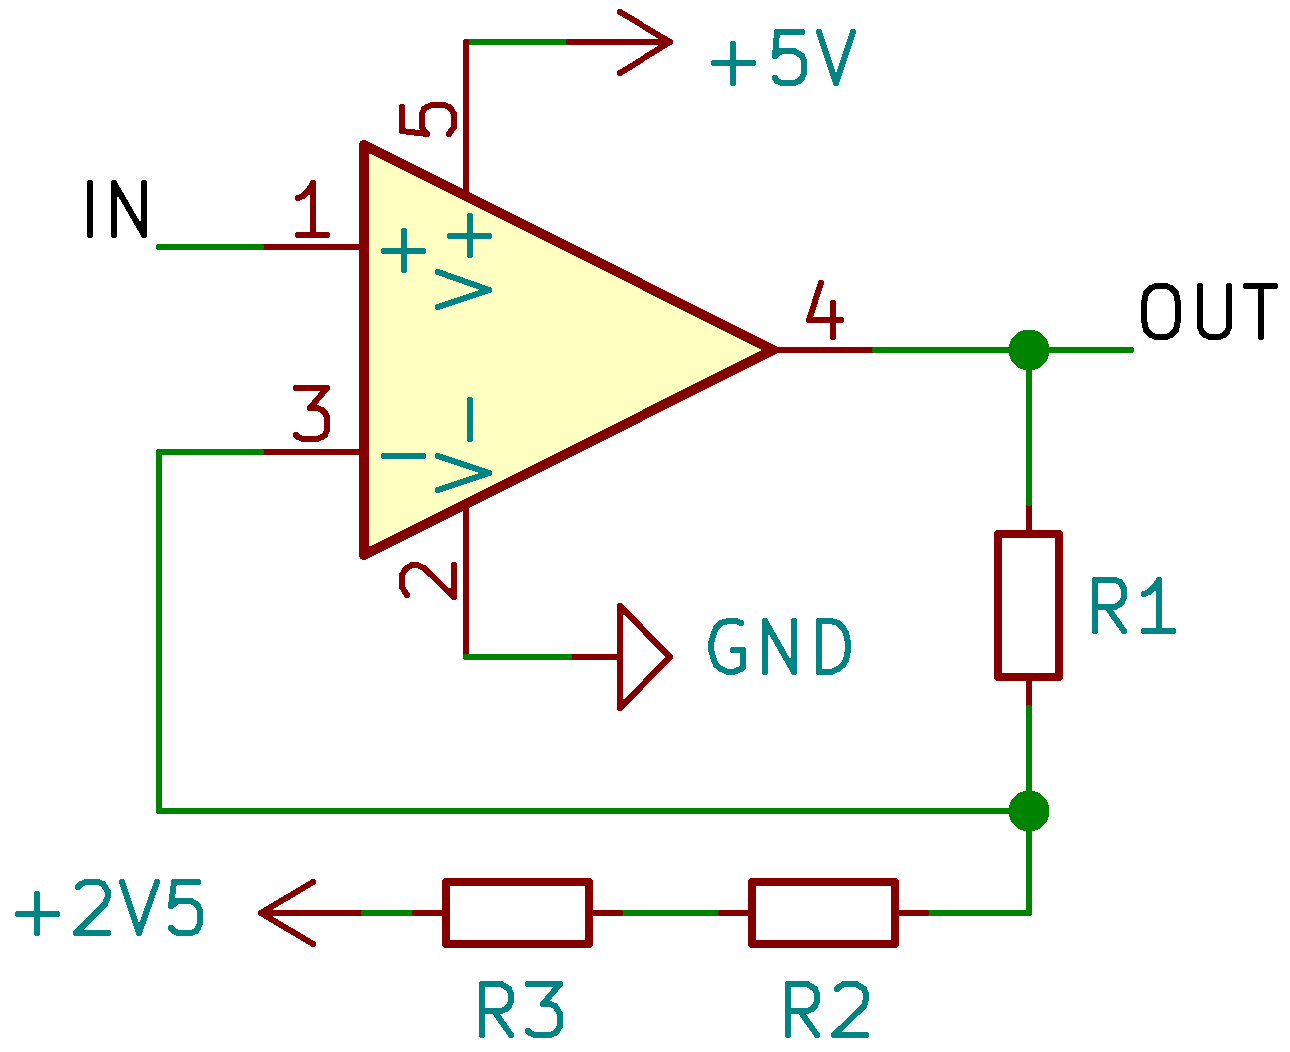
\includegraphics[width=\textwidth]{gain_circuit}
	\caption{The non-inverting amplifier circuit.}
	\label{fig:non-inverting-op-amp}
\end{subfigure}
\hfill
\begin{subfigure}[c]{0.45\textwidth}
	\centering
	\vfill
	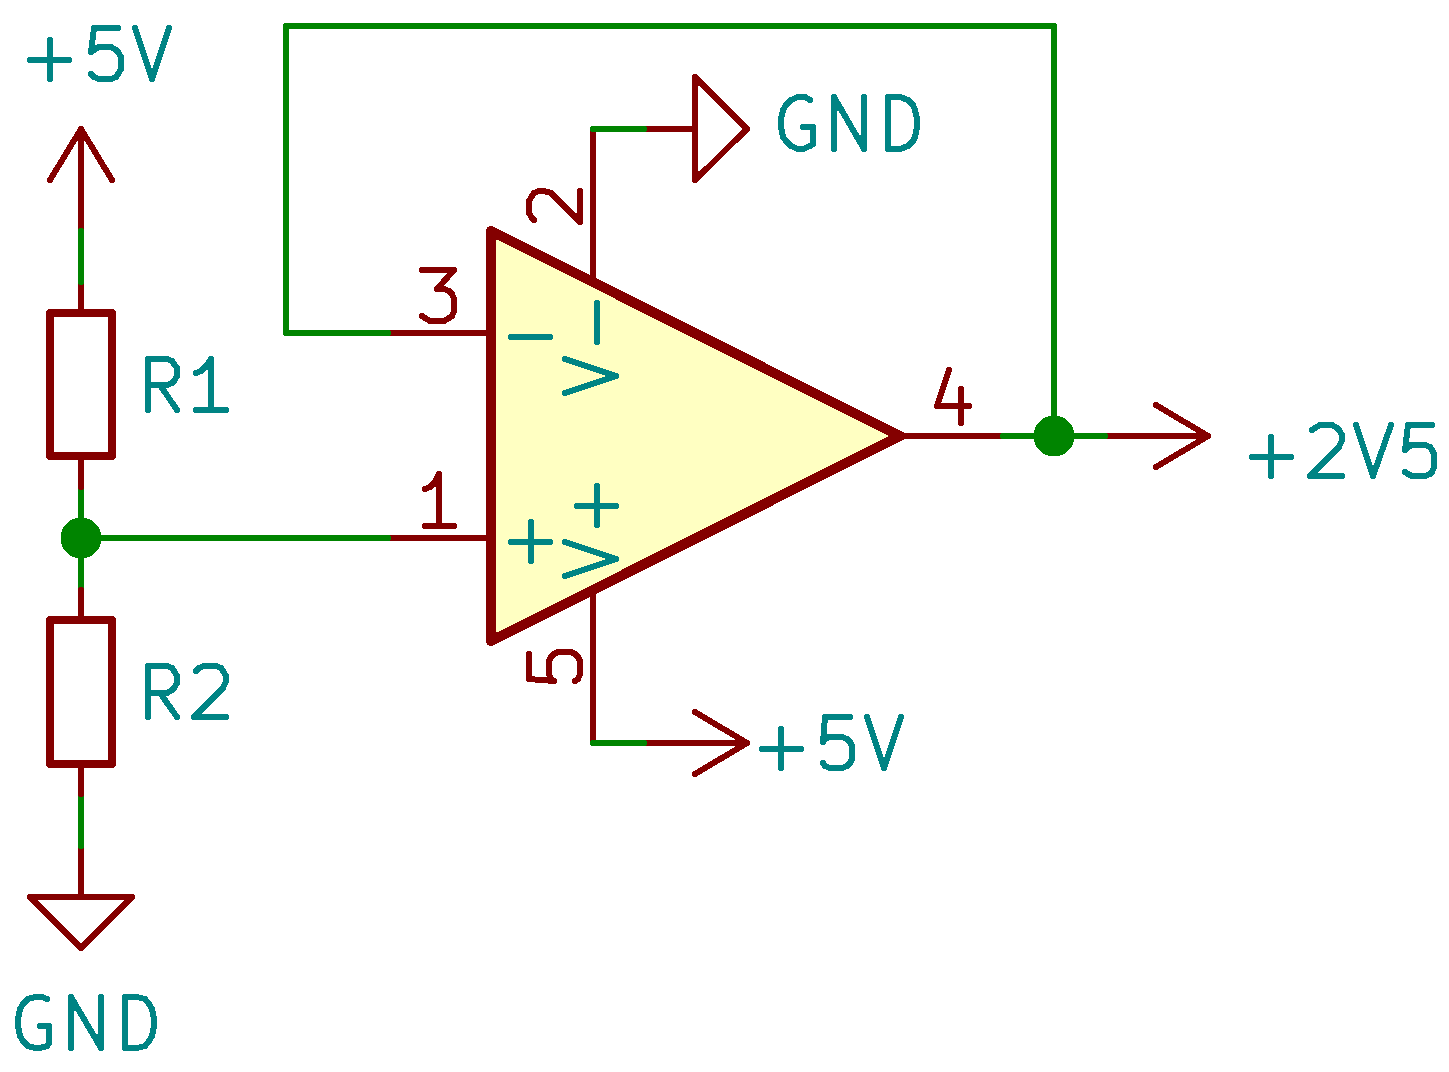
\includegraphics[width=\textwidth]{virtual_ground_circuit}
	\vfill
	\caption{The virtual ground circuit.}
	\label{fig:half-supply}
\end{subfigure}

\caption{The operational amplifer circuits used.}
\end{figure}

The op-amps were required to switch to a low power mode when no ADC readings are taking place.
The project requirements favour greater control over which op-amps can be turned on and off.
Due to our op-amp selection, they must be turned off in blocks of 4.
Therefore, it was decided that a CMOS inverter IC be used to drive the positive supply rail to ground.
The main drawback of this method is the start-up time to enable the op-amps.
The sum of the time taken to switch the op-amp back on is $\SI{50}{\micro\second}$ (this is a phase angle of $\SI{7.2}{\degree}$ with respect to the AC signal).

\subsubsection{Filtering Stage}

A low-pass filter circuit was designed to attenuate frequencies above $\SI{400}{\hertz}$.
This was done with a simple RC filter circuit (figure \ref{fig:filter}) because the cut-off frequency is less than $\SI{100}{\kilo\hertz}$.
The filter was designed to have a cut-off frequency of $\SI{600}{\hertz}$ so that frequencies above $\SI{400}{\hertz}$ would be attenuated.
The component values were $C = \SI{0.47}{\micro\farad}, R = \SI{560}{\ohm}$.

A drawback of this filter is that the output voltage is $V_{in} \sqrt{2}$, however it is required due to the type of ADC.
In this case, the maximum voltage the filter can output is $\SI{3.54}{\volt}$.
To acheive maximum output of $\SI{5}{\volt}$, the gain of the amplifier stage would need to be $141$ and the voltage would need to have a $\pm\SI{3.54}{\volt}$ range, centered around $\SI{2.5}{\volt}$.
Due to the requirements, this is not possible as the output voltage of the amplifier saturates at the supply rail voltage.

\subsubsection{Sampling Stage}

The sampling is done using a 12-bit successive approximation (SAR) ADC on the microcontroller.
The SAR hardware is accurate up to high resolutions but requires a stable input, hence the need for an RC filter.
All 12 ADCs exist as different channels on the same ADC peripheral and direct memory acccess (DMA) can be used to move the data to memory.
The ADC peripheral features a hardware averaging circuit which can be leveraged to reduce the load on the microcontroller core.




\subsection{Microcontroller}
\label{sec:microcontroller}

A 32-bit microcontroller (MCU) with at least 12 12-bit ADCs was required to communicate the current readings to the masterboard.
This MCU must communicate with masterboard to send readings every $\SI{100}{\milli\second}$.
Each slave must be time-synced with all other slaves with a deviation of no more than $\SI{1}{\micro\second}$.
The MCU must also be able to withstand temperatures of up to $\SI{105}{\degreeCelsius}$ and have support for the CAN protocol.

To meet these requirements the MKE16Z32VLD4 was chosen.
It has an ARM Cortex-M0+ core, a $\SI{48}{\mega\hertz}$ internal clock, $\SI{32}{\kilo\byte}$ of FLASH memory, and 12 SAR ADCs.
It is also able to run in environments of up to $\SI{105}{\degreeCelsius}$ and has a small 44-pin LQFP footprint.

Its hardware CAN support also requires an external CAN receiver.
This is discussed in section \ref{sec:communications}.




\subsection{Communications}
This section describes the top-level design. Key details can be found in appendix \ref{ap:communications}.

\subsubsection{Master to Daughterboards} 
Given the timing constraints, number of devices and environmental conditions, the evaluation process identified CAN bus and I2C as suitable communications systems.
CAN was chosen primarily due to its differential signalling mechanisms providing inbuilt noise immunity and upper protocol support. 

\subsubsection{Selection process}
Selection criteria were 1. number of devices supported, 2. raw data rate, 3 physical implementation, .1 connector requirements, .2 noise immunity, .3 ease of cabling installation and maintenance .4 supported topology. 
1. Systems supporting less than 127 devices were excluded.

2 raw speed / goodput
Systems with a raw data rate less than 128.32 kilobits per second were excluded.

3 physical
.1 Connectors
Systems with protocol or implementation specific connectors were excluded.
.2 Noise immunity 
Systems without inbuilt noise immunity and error checking were excluded.
.3 Ease of cabling / installation / maintenance 
Multidrop systems were favoured.
.4 Topology 
Systems that support multiple topologies were preferred.

\subsubsection{CAN transceiver selection}


\subsubsection{CAN bus physical implementation }
Separate cabling is used for data communications to meet the timing and signalling requirements of 1uSec and 100 mSec.

30AWG ribbon cable is used for reliability and ease of installation and maintenance since the bus is not broken per daughterboard, whilst meeting the timing requirements. Additionally, there is a greater range of 10 conductor options (compared to 8, 6 or 4 way) which also provides for dual bus expansion options. Strain relief is also provided with the chosen connector system. To provide maximum noise immunity and cable reversal protection the 10 conductors are arranged 00 AA 00 BB 00 where 0 represents signal ground, AA and BB are the two independent CAN signals. 


\subsubsection{Master to data logger}


\subsection{PCB Layout}
\label{sec:pcb-layout}

Careful consideration of the physical layout of the components on the printed circuit board (PCB) is important to reduce noise on the sensitive analog components.
Figure \ref{fig:layout} depicts the position of the components on the board.
Note the placement of the power electronics is away from the analog electronics and communications circuitry.

The PCB (figure \ref{fig:pcb-layout}) was designed in KiCAD.
The dimensions of the resulting board are $\SI{58}{\milli\metre}\times\SI{30}{\milli\metre}$, this is below the absolute maximum of $\SI{62}{\milli\metre}\times\SI{38}{\milli\metre}$.
\begin{figure}[H]
	\centering
	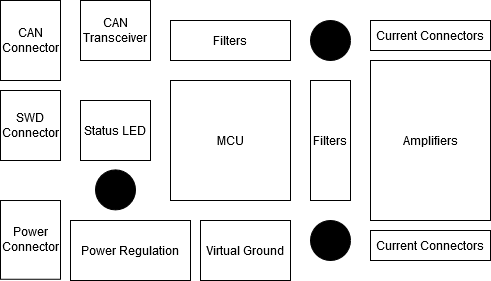
\includegraphics[width=0.8\textwidth]{layout}
	\caption{The approximate layout of the PCB.}
	\label{fig:layout}
\end{figure}

\begin{figure}[H]
	\centering
	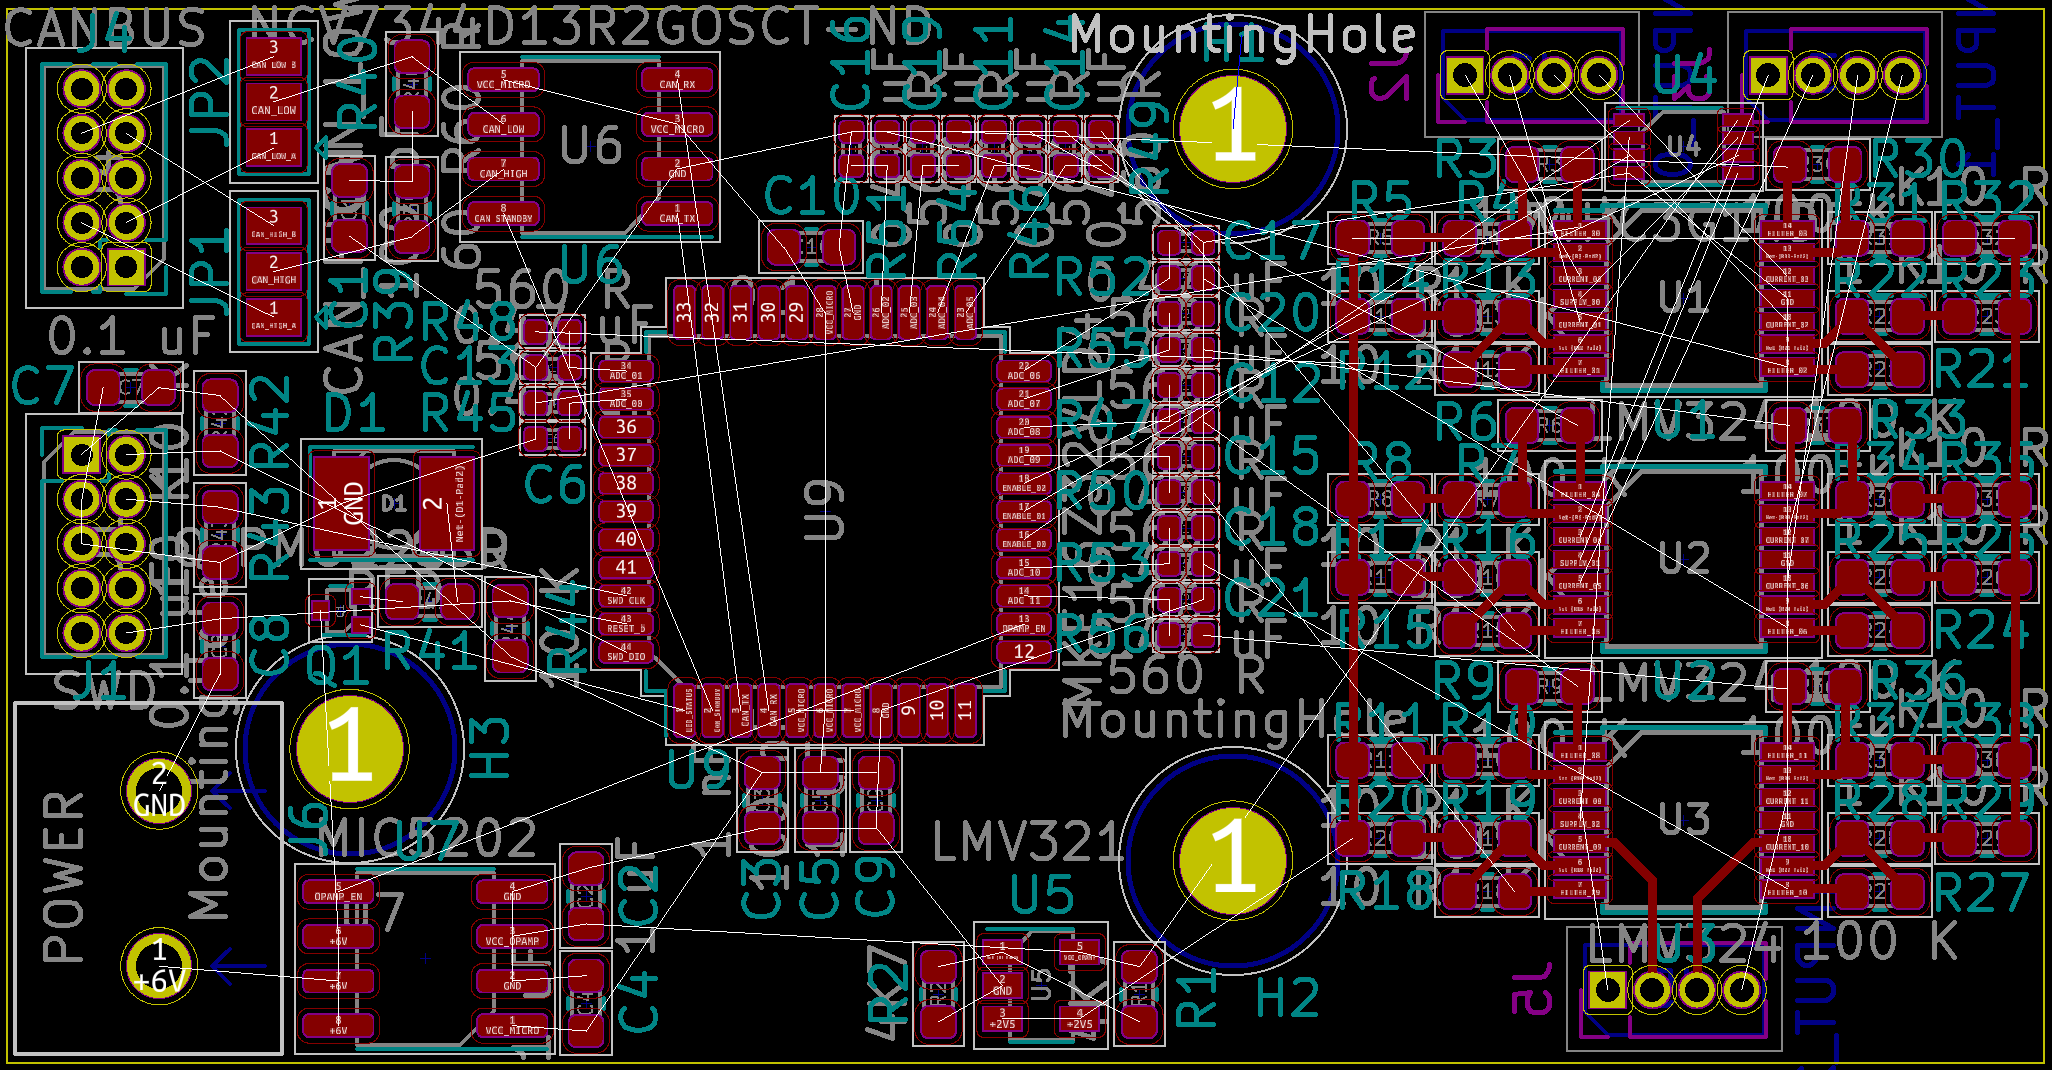
\includegraphics[width=\textwidth]{pcb_layout}
	\caption{The PCB layout viewed in KiCAD.}
	\label{fig:pcb-layout}
\end{figure}

% talk about the connectors to the motherboard
Three $\SI{2}{\milli\metre}$ diameter mounting holes are provided to aid in mounting the slave board on the motherboard.
The slave board would sit upon standoffs mounted to the motherboard using these mounting holes.
Three $\SI{1.27}{\milli\metre}$ pitch pin sockets connect the rear side of the PCB to the motherboard, either via short cables or a pin header arrangement.
The goal of this is to offer different mounting and connection options.




\section{Conclusion}

A daughter-board was designed to take ADC readings from a current transducer within a thermally and electrically noisy environment.
Operational amplifiers were used to amplify the sensor voltages and low-pass RC filters were used to condition the signals.
A microcontroller was used to quantise the analog readings into a form that can be further conditioned in software.
A CAN transceiver was used to transmit the data to a master-board where the data is collated and sent to a data-logger via the 802.11b/g/n protocol.


%%%%%%%%%%%%%%%%%%%%%%%%%%%%%%%%%%%%%%%%%%%%%%%%%%%%%%%%%%%%%%%%%%%%%%%%%%%%%%%%
%%%%%%%%                           BIBLIOGRAPHY                         %%%%%%%%
%%%%%%%%%%%%%%%%%%%%%%%%%%%%%%%%%%%%%%%%%%%%%%%%%%%%%%%%%%%%%%%%%%%%%%%%%%%%%%%%

\printbibliography

% appendix
\newpage
\appendix

\subsection{Conditioning}
\label{ap:conditioning}

The input impedance and gain for the non-inverting amplifier circuit are given by equations \ref{eq:zi} and \ref{eq:gain} respectively.
\begin{align}
	Z_i &= \frac{R_1 (R_2 + R_3)}{R_1 + R_2 + R_3} \label{eq:zi} \\
	A_v &= 1 + \frac{R_1}{R_2 + R_3}\label{eq:gain}
\end{align}

The source impedance is specified as being less than $\SI{100}{\ohm}$.
A input impedance that is at least an order of magnitude higher than the source impedance is required for maximum voltage transfer and minimum current drain.
$Z_i = \SI{1}{\kilo\ohm}$ was decided upon, because it is 10 times higher than the worst-case source impedance.
Equations \ref{eq:r1} and \ref{eq:r2} show the derived formulae for the resistors based upon the given $Z_i$ and $A$ values.
\begin{align}
	R_1 &= Z_i A \label{eq:r1} \\
	R_2 + R_3 &= \frac{Z_i A}{A - 1} \label{eq:r2} \\[1em]
	\therefore R_1 = \SI{130}{\kilo\ohm}, R_2 &= \SI{920}{\ohm}, R_3 = \SI{8.2}{\ohm} \nonumber
\end{align}

Thermal calculations (\textcolor{red}{add reference to appendix}) show that the op-amps will supply minimal current into the microprocessor's ADC inputs.
Thus their power dissapation is relatively low.
The power dissapation is a function of the difference between supply voltage to output voltage, output voltage difference to ground (for single supply devices) and the output current.
With low power dissapation, there is a comfortable margin between the ambient temperature of $\SI{105}{\degreeCelsius}$, the junction operating temperature of $\SI{125}{\degreeCelsius}$, and the device absolute maximum of $\SI{150}{\degreeCelsius}$.
Additionally the worst case quiescent current is $\SI{150}{\micro\ampere}$.



\end{document}
